\documentclass{article}
\usepackage{ctex}
\usepackage{graphicx}
\usepackage{amsmath}
\usepackage{indentfirst}
\usepackage{titlesec}
\usepackage{setspace}
\usepackage{subfigure}
\usepackage{caption}
\usepackage{float}
\usepackage{booktabs}
\usepackage{geometry}
\usepackage{multirow}
\geometry{left=2cm,right=2cm,top=2cm,bottom=2cm}
\title{\songti \zihao{2}\bfseries 底心正交晶体性质小论文}
\titleformat*{\section}{\songti\zihao{4}\bfseries}
\titleformat*{\subsection}{\songti\zihao{5}\bfseries}
\renewcommand\thesection{\arabic{section}}
\author{王启骅 PB20020580}
\begin{document}
	\maketitle
	\section{结构}
	文章将会讨论底心正交晶体的一些结构与性质。首先底心正交晶体布拉维格子的结构如图1所示,设定三边分别为$ a_1,a_2,a_3 $,且根据定义,$ a_1\neq a_2\neq a_3 $,三边相互垂直。假设$ a_1<a_2<a_3 $。
	\begin{figure}[!h]
		
		\centering
		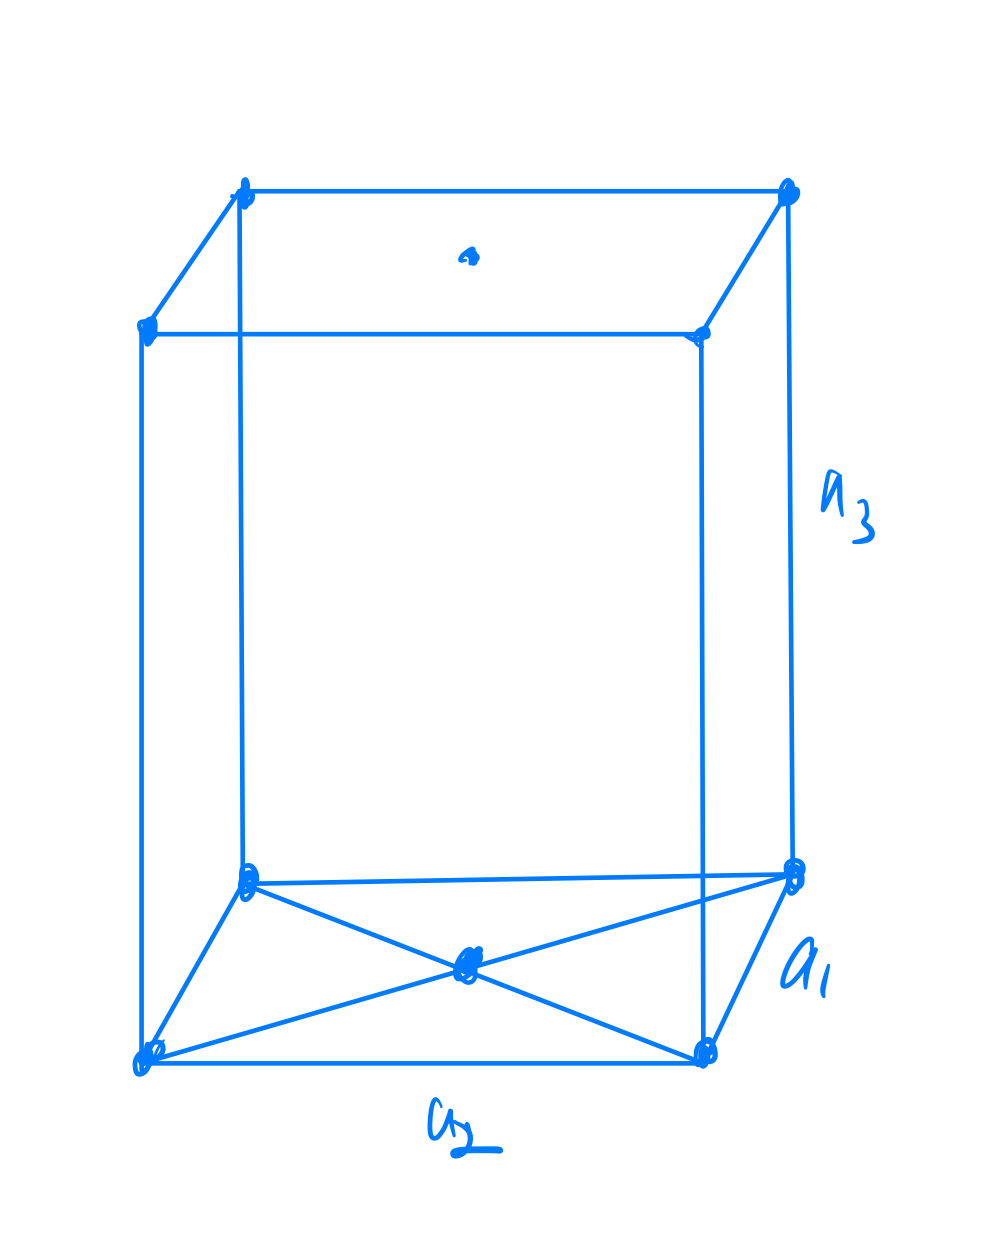
\includegraphics[scale=0.2]{1}
		\captionsetup{font={small},labelfont=bf}
		\caption{\heiti\zihao{-5}底心正交晶体布拉维格子}
		
	\end{figure}
	
	
	通过底心点到最近点(底面另不共线两点与上底心)的连线,可以得到原胞结构如图2,实际上该原胞其与单斜晶体唯一的不同就是底面的两边相等。
		\begin{figure}[!h]
		
		\centering
		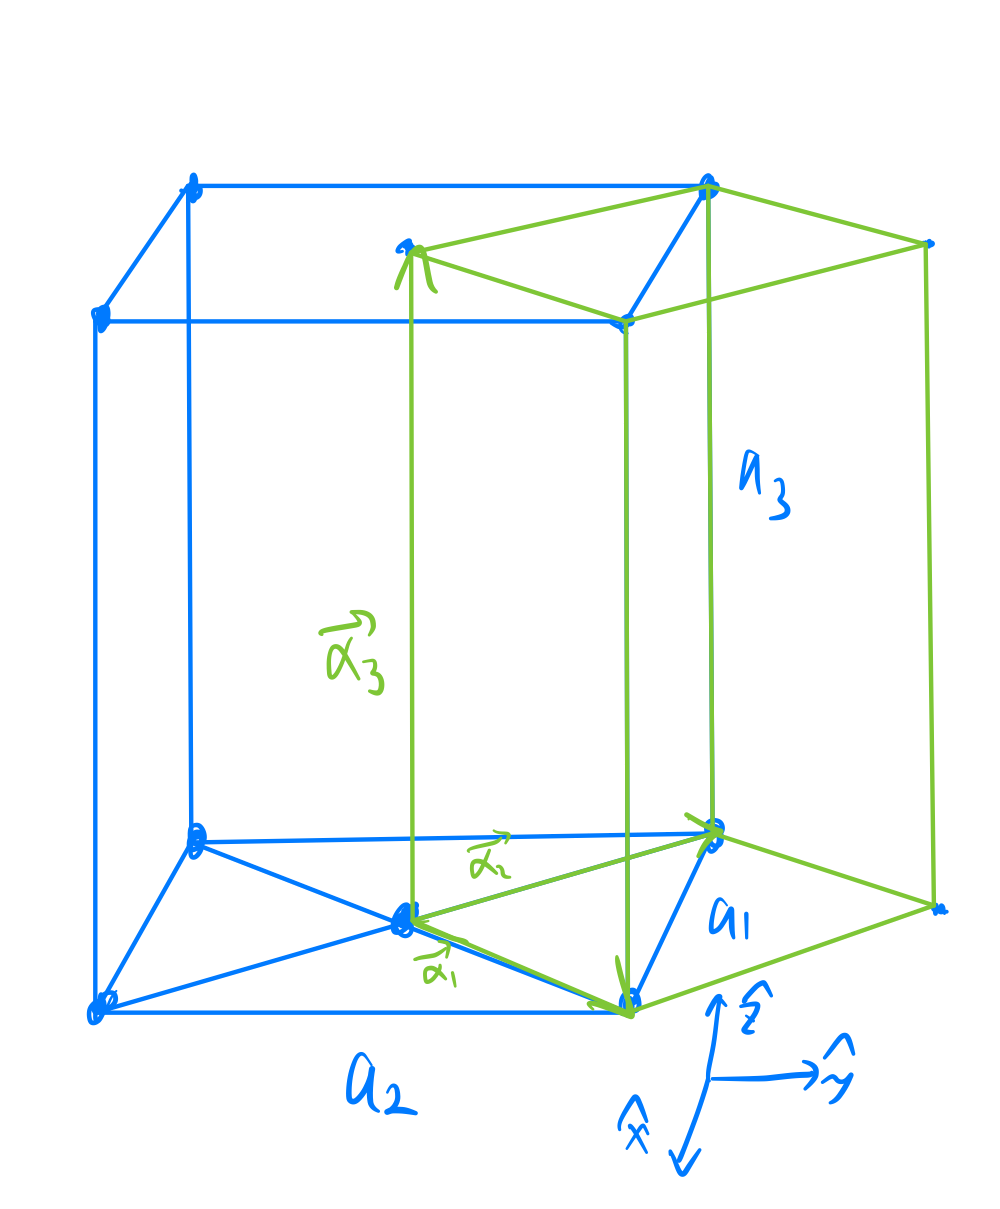
\includegraphics[scale=0.2]{原胞}
		\captionsetup{font={small},labelfont=bf}
		\caption{\heiti\zihao{-5}底心正交晶体原胞}
		
	\end{figure}
可得原胞基矢为
 \begin{equation}
 	\begin{cases}
 		\vec{\alpha_1}=\frac{a_1}{2}\hat{x}+\frac{a_2}{2}\hat{y}\\
 		\vec{\alpha_2}=-\frac{a_1}{2}\hat{x}+\frac{a_2}{2}\hat{y}\\
 		\vec{\alpha_3}=a_3\hat{z}
 	\end{cases}
 \end{equation}
	
	
	也可以得到底心正交晶系的Wigner-Seitz原胞。首先绘制布拉维格子的俯视图如图3(a),将底心点与周围最近点的连线作垂直平分线后划分出的区域。可得由于底心正交晶格的底面为不等边的矩形,故底心与最近各点的连线的中垂线必定会在矩形较长边切出一条边,形成一个六边形。之后再扩展到三维,将与上下底心连线的中垂面做出,即可得到其WS原胞为一个六边形柱体。

\begin{figure}[!h]
	\centering
	\subfigure[WS原胞俯视图]{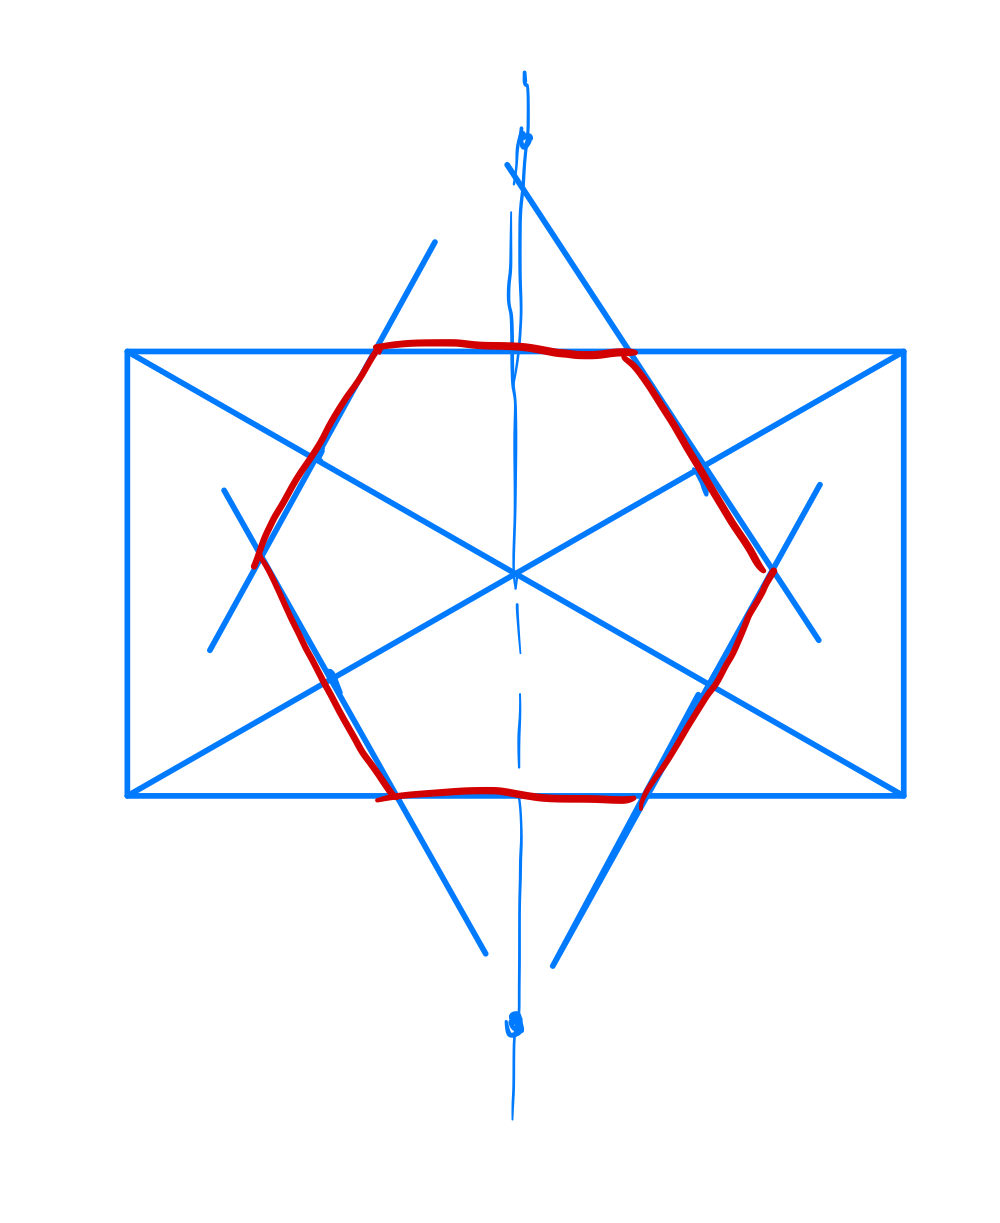
\includegraphics[scale=0.15]{WS俯视图}}
	\subfigure[WS原胞]{	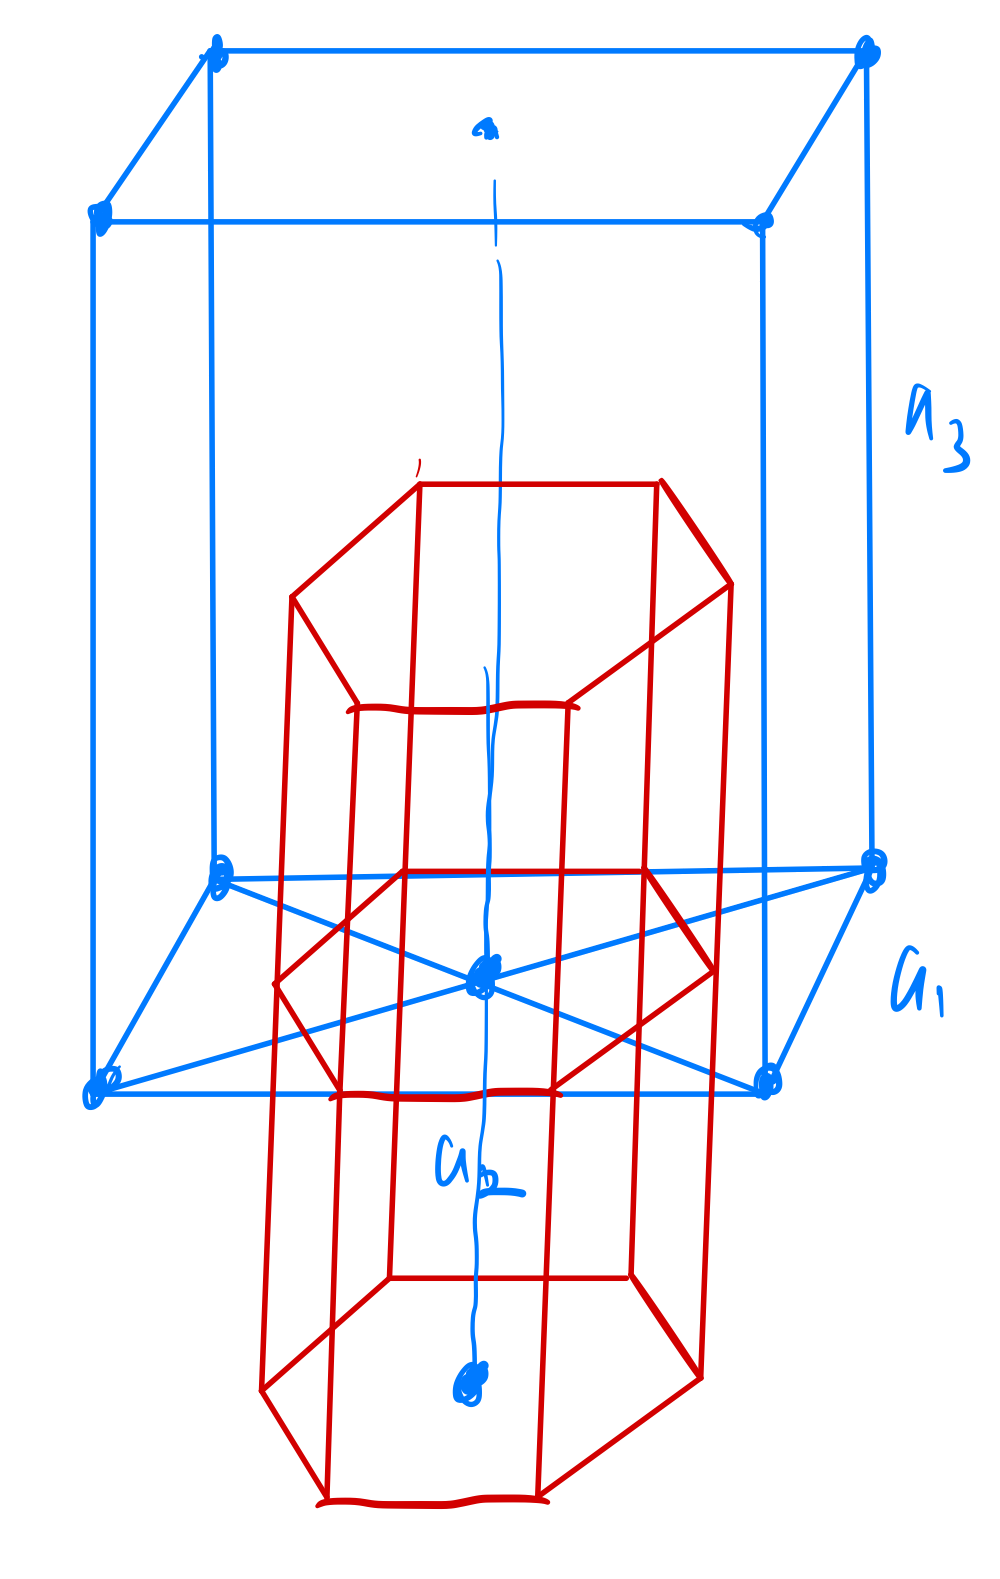
\includegraphics[scale=0.15]{WS原胞}}
	\captionsetup{font={small},labelfont=bf}
	\caption{\heiti\zihao{-5}Wigner-Seitz原胞}
	
\end{figure}
\section{对称性}
\begin{figure}[!h]
	\centering
	\subfigure[对称轴]{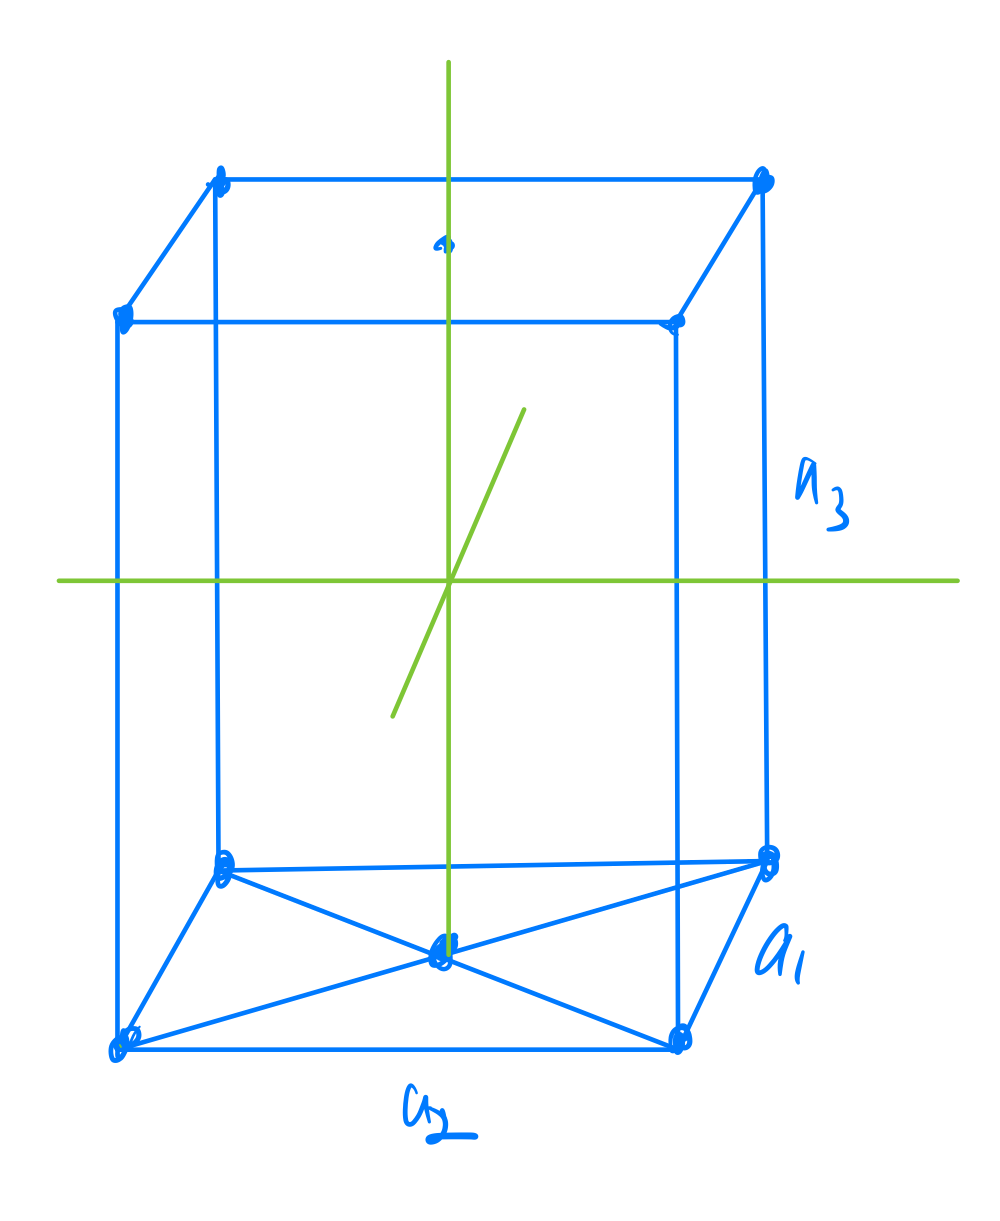
\includegraphics[scale=0.15]{对称轴}}
	\subfigure[对称面]{	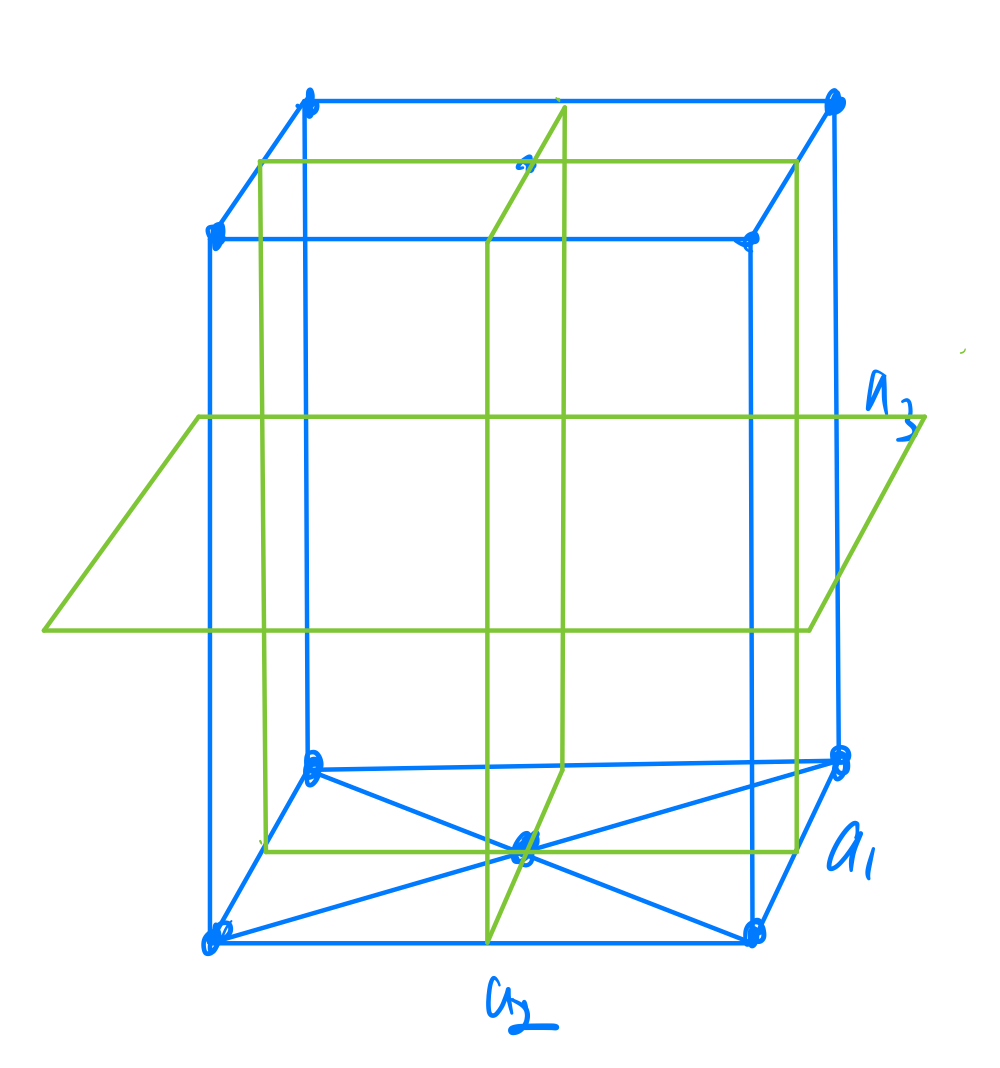
\includegraphics[scale=0.15]{对称面}}
	\captionsetup{font={small},labelfont=bf}
	\caption{\heiti\zihao{-5}对称性}
	
\end{figure}
首先该底心正交晶体满足相对于六面体心反演对称。


底心正交晶体的对称轴如图4(a)所示,上下底心的连线为一个二次旋转对称轴,垂直于该二次旋转对称轴有两个沿x、y方向的二次旋转对称轴。由此说明晶格属于$ D_2 $群。


同时如图4(b)可得上下底心连线的中垂面,和法向量沿x、y的两个面都为该晶格的反映面。其中一个面垂直于二重轴,两个面包含二重轴。由此可得晶格也属于$ C_{2v} $与$ D_{2h} $群。

\section{倒易点阵与布里渊区}
	\begin{figure}[!h]
	
	\centering
	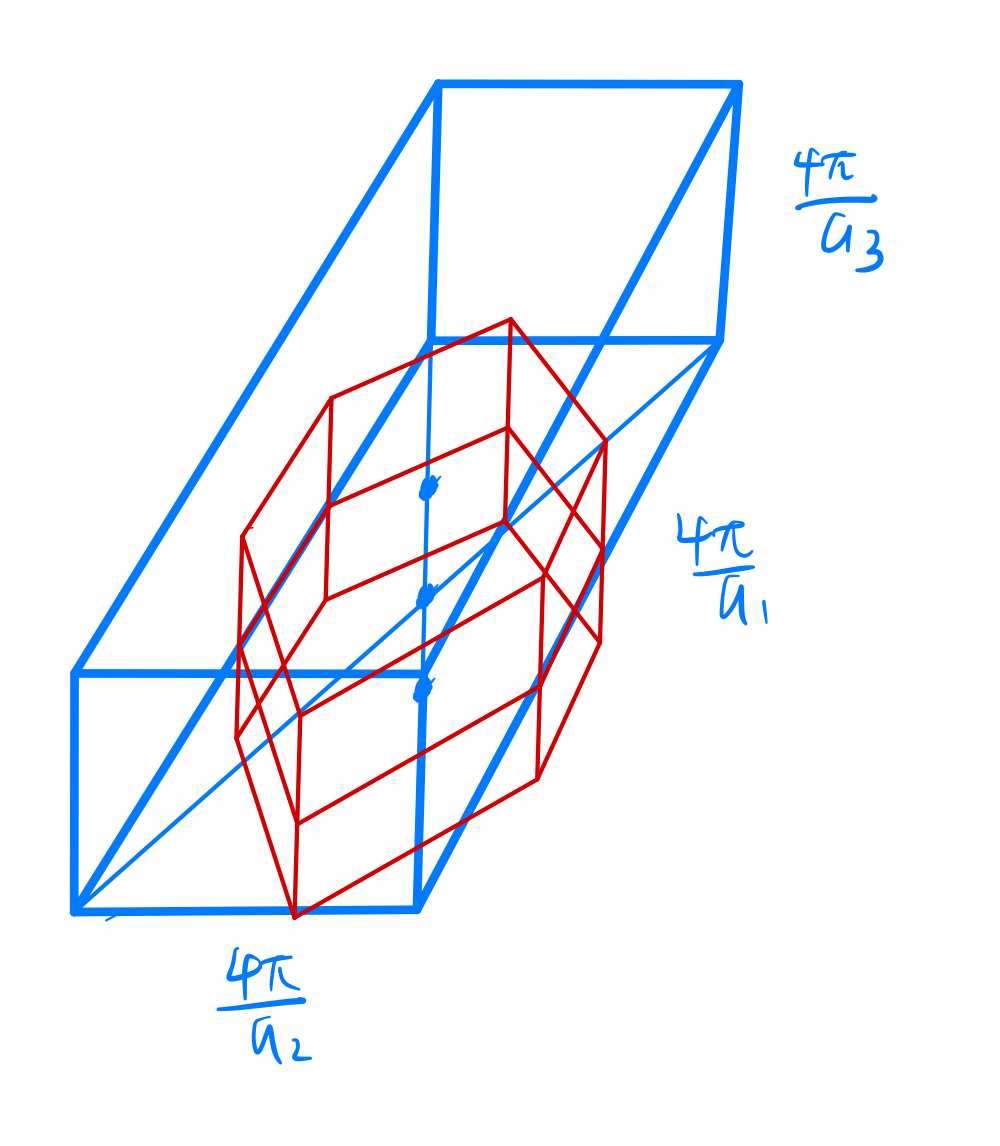
\includegraphics[scale=0.2]{布里渊区}
	\captionsetup{font={small},labelfont=bf}
	\caption{\heiti\zihao{-5}底心正交晶体布里渊区}
	
\end{figure}
以下计算底心正交晶体的倒易点阵基矢。首先有
\begin{equation}
	\vec{\alpha_1}\cdot[\vec{\alpha_2}\times\vec{\alpha_3}]=\frac{a_1a_2a_3}{2}
\end{equation}
则
\begin{equation}
	\begin{cases}
		\vec{b_1}=2\pi\frac{\vec{\alpha_2}\times\vec{\alpha_3}}{\vec{\alpha_1}\cdot[\vec{\alpha_2}\times\vec{\alpha_3}]}=\frac{2\pi}{a_1a_2}(a_2\hat{x}+a_1\hat{y})\\
		\vec{b_2}=2\pi\frac{\vec{\alpha_3}\times\vec{\alpha_1}}{\vec{\alpha_1}\cdot[\vec{\alpha_2}\times\vec{\alpha_3}]}=\frac{2\pi}{a_1a_2}(-a_2\hat{x}+a_1\hat{y})\\
		\vec{b_3}=2\pi\frac{\vec{\alpha_1}\times\vec{\alpha_2}}{\vec{\alpha_1}\cdot[\vec{\alpha_2}\times\vec{\alpha_3}]}=\frac{2\pi}{a_3}\hat{z}
	\end{cases}
\end{equation}
由此可见,底心正交晶体的倒格子仍为底心正交点阵,三边边长分别变为$ a_1\rightarrow\frac{4\pi}{a_1} ,a_2\rightarrow\frac{4\pi}{a_2},a_3\rightarrow\frac{4\pi}{a_3}$。绘制出其倒格子,并按照相同的方法绘制出了布里渊区如图5。由于三边再倒格子后相对长度相反,则在倒格子的WS原胞中,六边形所截的边为原来较短边$ a_1 $所对应的边。

\section{总结}
文章讨论了底心正交晶体的一些结构、原胞、对称性、倒易点阵与布里渊区等性质。由于各个边相互垂直,该晶格有一定较好的性质与对称性,但是由于各边长度的不相等,其对称性等又稍逊于四方、立方等晶系。
\end{document}